\chapter{Introduction}
\section{Logistics}
\begin{minipage}{.3\textwidth}
    \begin{center}
        \begin{tikzpicture}
            \clip (0,0)  circle (2cm) ;
            \node[anchor=center] at (0,-0.5) {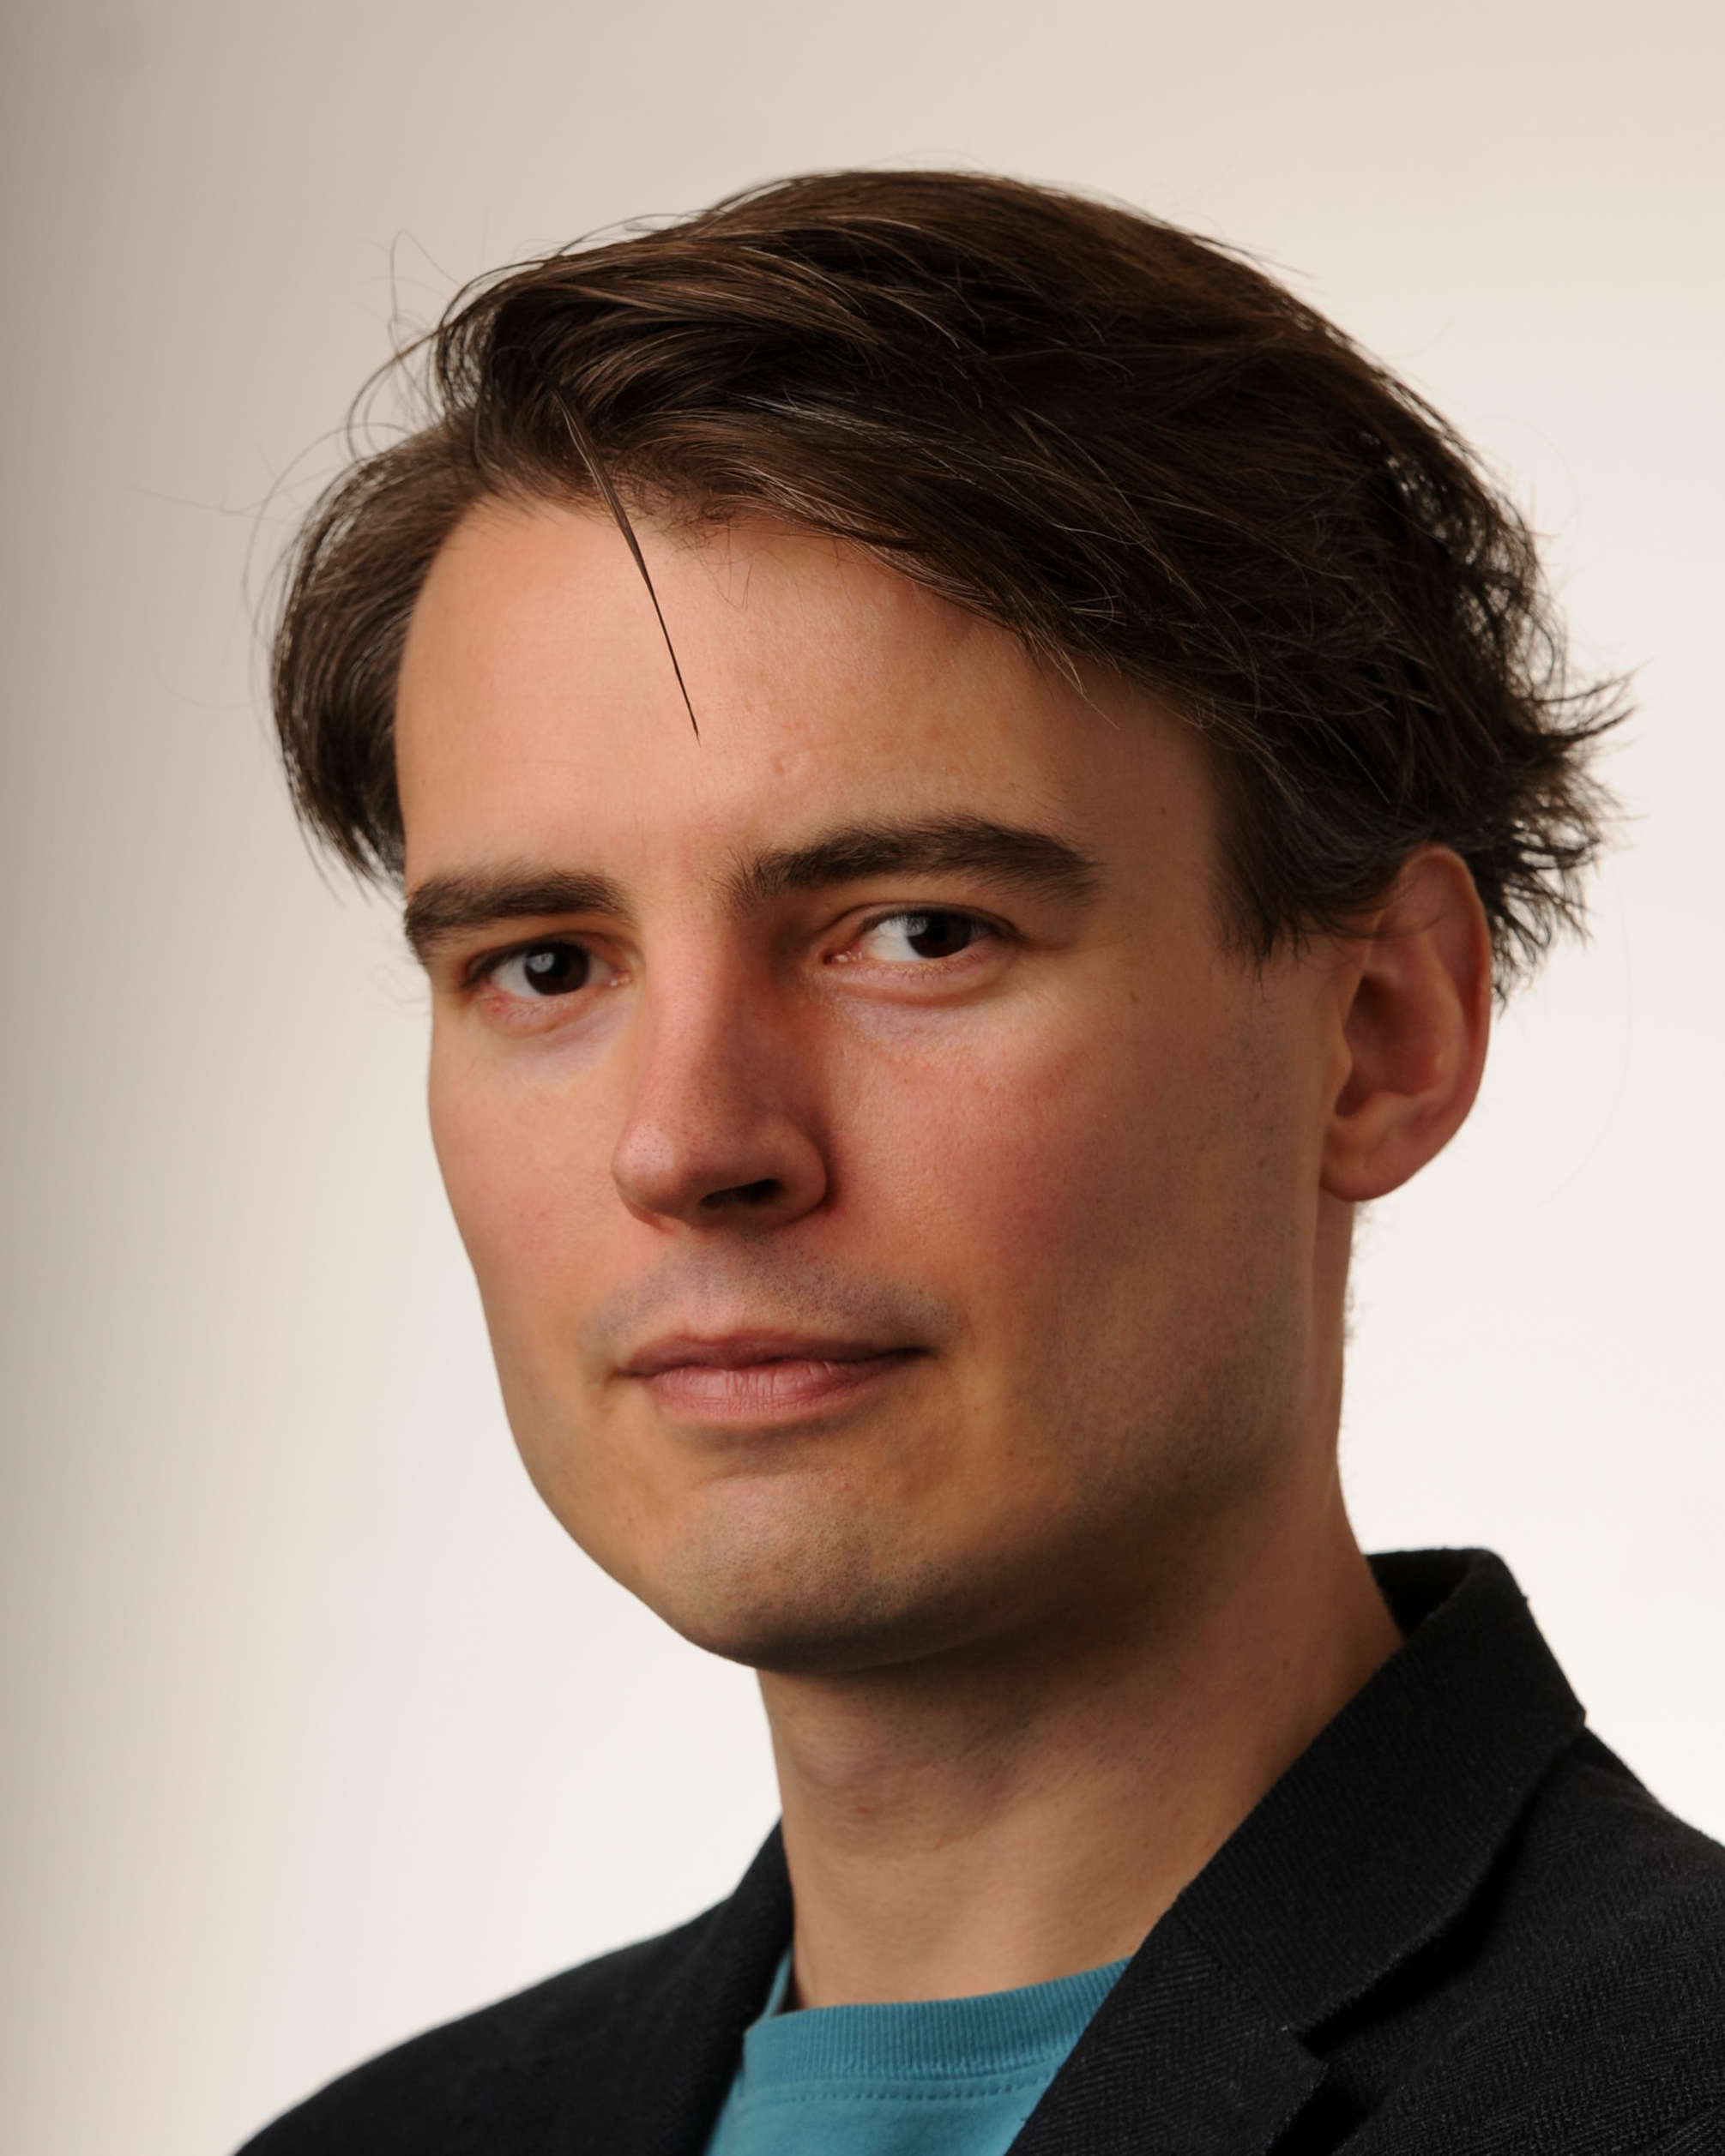
\includegraphics[width=4.5cm]{introduction/images/holger_pirk.jpg}};
        \end{tikzpicture}
        \centerline{\textbf{Dr Holger Pirk}}
    \end{center}
\end{minipage} \hfill \begin{minipage}{.65\textwidth}
    The module is taught by \href{https://holger.pirk.name/}{Dr Holger Pirk}.
    \begin{itemize}
        \item Taught as prerecorded lectures with in-person Q\&As
        \item Weekly tutorial sheets covered during the Q\&A sessions
        \item One coursework in teams of 3 (with a competition!)
    \end{itemize}
\end{minipage}
\subsection{SQL}
\begin{center}
    \textbf{SQL is not prerequisite for this course!}
\end{center}
The \href{https://www.doc.ic.ac.uk/~pjm/idb/}{\textbf{40007 - Introduction to Databases}} module covers all that is required. This module is about the implementation of data processing systems, not using databases \& SQL.

\subsection{C++}
\begin{center}
    \textbf{C++ is not prerequisite for this course!}
\end{center}
This course contains many code examples in C++. This course represents a great
opportunity to learn at least a small part of its enormity, and to apply some of this
in the coursework.
\begin{sidenotebox}{C++ $>$ C with classes}
    C++ was originally developed around 1983 by Bjarne Stroustrup as \textit{'C with classes'} and implemented as a transpiler to C called cfront.
\end{sidenotebox}
\noindent \twosplit{
    \begin{center}
        
\includegraphics[height=3cm]{introduction/images/cppreference.jpg}
        \\ \href{https://en.cppreference.com/}{\textbf{CppReference}}
        \\ \textit{Comprehensive C++ and standard template library documentation.}
    \end{center}
}{
    \begin{center}
        
\includegraphics[height=3cm]{introduction/images/cmake.png}
        \\ \href{https://cmake.org/cmake/help/book/mastering-cmake/index.html}{\textbf{Mastering CMake}}
        \\ \href{https://cmake.org/cmake/help/latest/}{\textbf{CMake Documentation}}
    \end{center}
}
\\ \twosplit{
    \begin{center}
        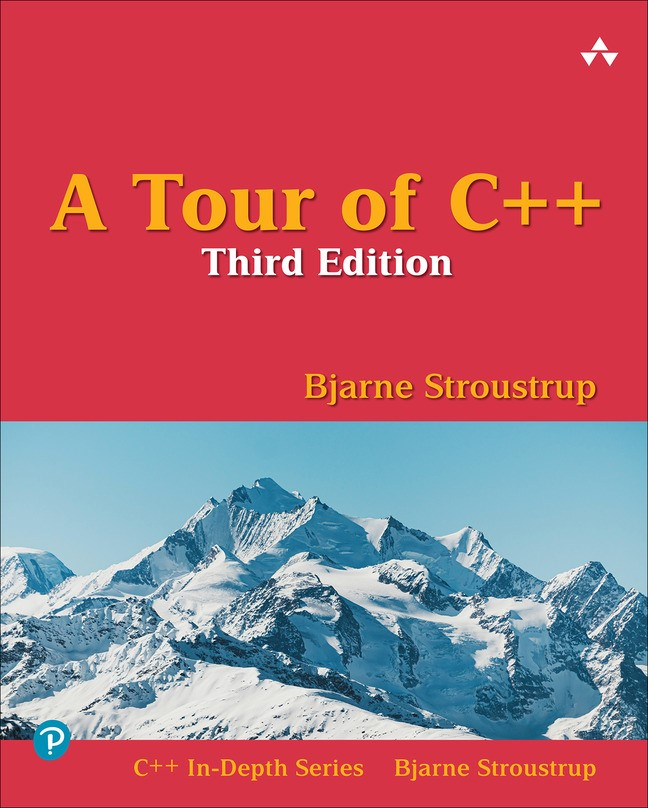
\includegraphics[height=6cm]{introduction/images/tour_of_cpp_3rd_ed.jpg}
        \\ \textbf{A tour of C++}
        \\ \textit{An overview of C++, only need C}
        \\ \textit{knowledge carried from pintos}
    \end{center}
}{
    \begin{center}
        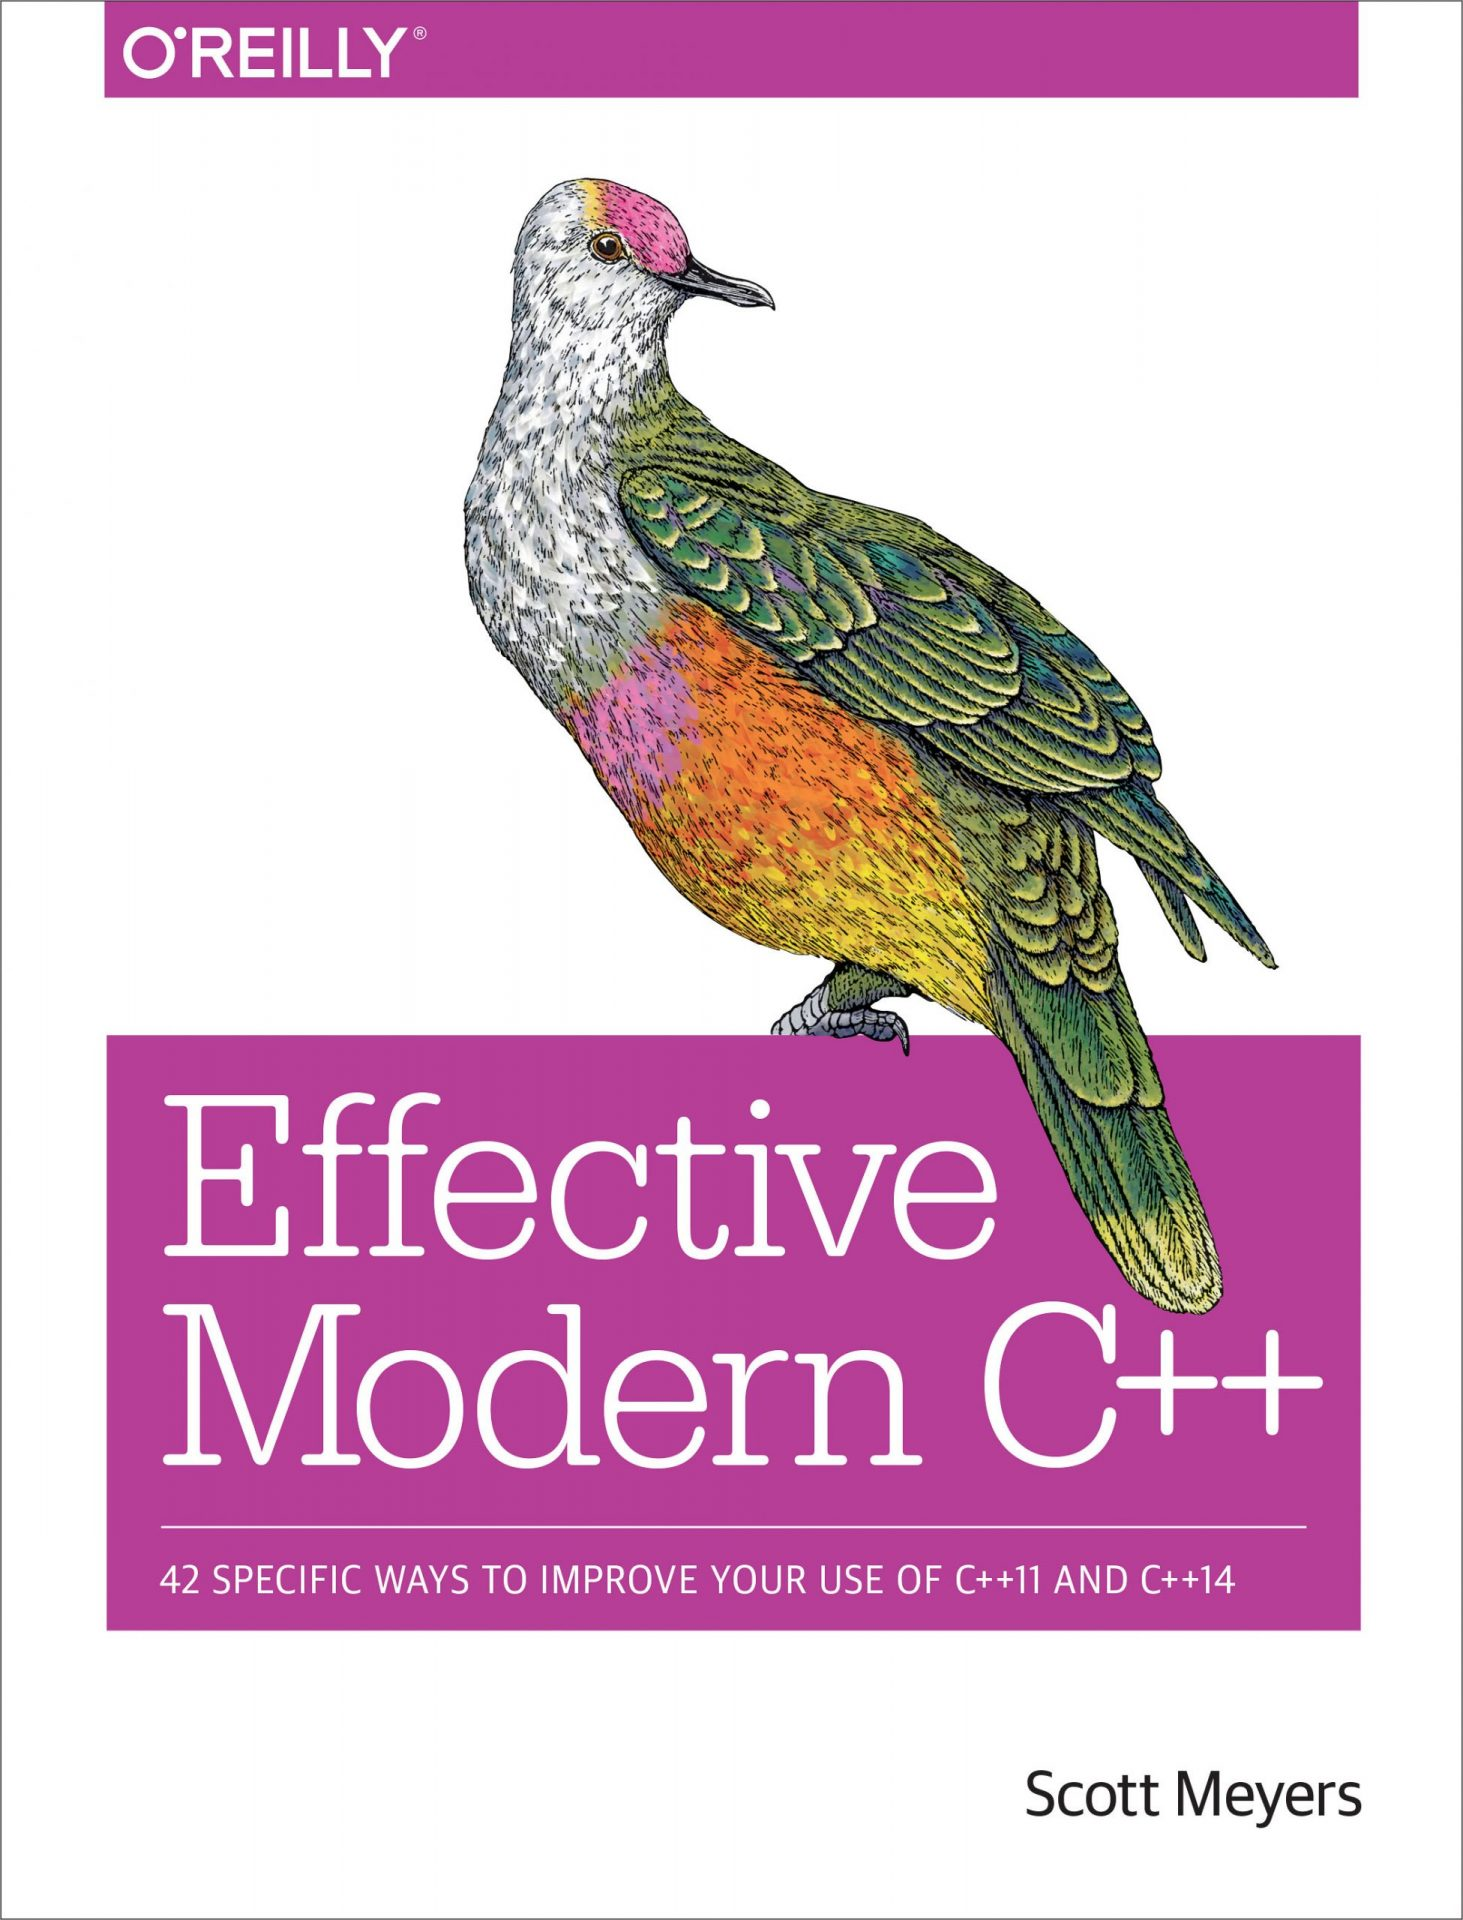
\includegraphics[height=6cm]{introduction/images/Effective-Modern-Cpp.jpg}
        \\ \textbf{Effective Modern C++}
        \\ \textit{modern C++ exploration \& best practices}
    \end{center}
}
\\ \vspace{5mm}
\\ The above books are available online from O'Reilly through Imperial (use institution login) for free \& you may find useful for learning more C++ (though beyond the understanding required for this module).

\section{Data Management Systems}
\begin{definitionbox}{Database}
    A large collection of organized data.
    \begin{itemize}
        \item Can apply to any structured collection of data (e.g a relational table, data structures such as vectors \& sets, graphs etc.)
    \end{itemize}
\end{definitionbox}

\begin{definitionbox}{System}
    A collection of components interacting to achieve a greater goal.
    \begin{itemize}
        \item Usually applicable to many domains (e.g a database, operating system, webserver). The goal is domain-agnostic
        \item Designed to be flexible at runtime (deal with other interacting systems, real conditions) (e.g OS with user input, database with varying query volume and type)
        \item Operating conditions are unknown at development time (Database does not know schema prior, OS does not know number of users prior, Tensorflow does not know matrix dimensionality prior)
    \end{itemize}
    Large \& complex systems are typically developed over years by multiple teams.
\end{definitionbox}

\begin{tcbraster}[raster columns=2, raster equal height]
    \begin{definitionbox}{Data Management System}
        A system built to control the entire lifecycle of some data.
        \begin{itemize}
            \item Creation, modification, inspection and deletion of data
            \item Classic examples include \textit{Database Management Systems}
        \end{itemize}
    \end{definitionbox}
    \begin{definitionbox}{Data Processing System}
        A system for processing data.
        \begin{itemize}
            \item Support part of the data lifecycle
            \item A strict superset of Data Management Systems (all data management systems are data processing systems)
        \end{itemize}
        For example a tool as small as \mintinline{bash}{grep} could be considered a data processing system.
    \end{definitionbox}
\end{tcbraster}
\noindent
Building data management systems is hard!
\begin{itemize}
    \item Often must fetch data continuously from multiple sources
    \item Needs to be highly reliable (availability/low downtime \& data retention)
    \item Needs to be efficient (specification may contain performance requirements)
\end{itemize}
\begin{center}
    \begingroup
    \setlength{\tabcolsep}{10pt} % Default value: 6pt
    \renewcommand{\arraystretch}{1.5} % Default value: 1
    \begin{tabular}{p{.25\textwidth} p{.75\textwidth}}
        \textbf{Storage}                                 & Needs to be persistent (but also needs to be fast)                                                                                                                   \\
        \textbf{Data Ingestions}                         & Needs to allow for easy import of data (e.g by providing a csv, another database's url)                                                                              \\
        \textbf{Concurrency}                             & To exploit parallelism in hardware (e.g multithreaded, distributed over several machines)                                                                            \\
        \textbf{Data Analysis}                           & For inspection (typically the reason to hold data in for first place)                                                                                                \\
        \textbf{User Defined Functions}                  & Needs to allow users to write their own queries on data.                                                                                                             \\
        \textbf{Standardized \newline Programming Model} & Features are not implemented in an ad-hoc way but through common abstractions, users and developers do not need to radically change how they approach a new feature. \\
        \textbf{Access Control}                          & Not all data is shared between all users.                                                                                                                            \\
        \textbf{Self-Optimization}                       & Monitors its own workloads in an attempt to optimise (e.g keeping frequently accessed data in memory)                                                                \\
    \end{tabular}
    \endgroup
\end{center}

\section{Data Intensive Applications}
\begin{definitionbox}{Data Intensive Application}
    An application the acquires, stores and processes a significant amount of information.
    Core functionality of the application is based on data.
\end{definitionbox}

\begin{definitionbox}{Online Transaction Processing (OTP)}
    \begin{center}
        \begin{tabular}{c c}
            High volume of small updates to a persistent database. & ACID is important. \\
        \end{tabular}
    \end{center}
    Goal: \textbf{Throughput}
\end{definitionbox}
\begin{definitionbox}{Online Analytical Processing (OLAP)}
    \begin{center}
        \begin{tabular}{c c c}
            Running a single data analysis task. & Mixture of query types. & Queries are ad-hoc. \\
        \end{tabular}
    \end{center}
    Goal: \textbf{Latency}
\end{definitionbox}
\begin{definitionbox}{Reporting}
    \begin{center}
        \begin{tabular}{c c c}
            Running a set of data analysis tasks. & Fixed time budget. & Queries known in advance. \\
        \end{tabular}
    \end{center}
    Goal: \textbf{Resource Efficiency}
\end{definitionbox}

\begin{examplebox}{Daily Struggle}
    Provide some examples of \textit{Reporting} pattern being used in industry.
    \tcblower
    \begin{itemize}
        \item A supermarket getting the day's sales, and stock-take.
        \item A trading firm computing their position and logging the days trades at market-close and informing regulators, clearing, risk department.
        \item A company's payroll systems running weekly using week long timesheets.
    \end{itemize}
\end{examplebox}

\subsubsection{Hybrid Transactional / Analytical Processing (HTAP)}
\begin{itemize}
    \item Small updates interwoven with larger analytics
    \item Need to be optimal for combination of small and large task sizes
\end{itemize}

\begin{sidenotebox}{HTAP}
    HTAP is a relatively new pattern used to solve the need for separate systems to work on OTP and OLAP workloads (which introduced complexity and cost as data is frequently copied between the two systems). Read more \href{https://en.wikipedia.org/wiki/Hybrid_transactional/analytical_processing}{here}.
\end{sidenotebox}
\noindent
\textit{Data-Intensive Applications} can be differentiated from \textit{Data Management Systems} (though there is ample ambiguity):
\begin{itemize}
    \item Applications are domain-specific, and hence contain domain-specific optimisations that prevent fully general-purpose usage
    \item Data Management Systems are required to be highly generalised
    \item The cost of application specific data management (e.g developer time) outweighs any benefits for the majority of cases
\end{itemize}

\begin{definitionbox}{Model View Controller (MVC)}
    A common design pattern separating software into components for user interaction (view), action (controller) and storing state (model) which interact.
\end{definitionbox}

A typical \textit{data intensive application} has the following architecture:
\begin{center}
    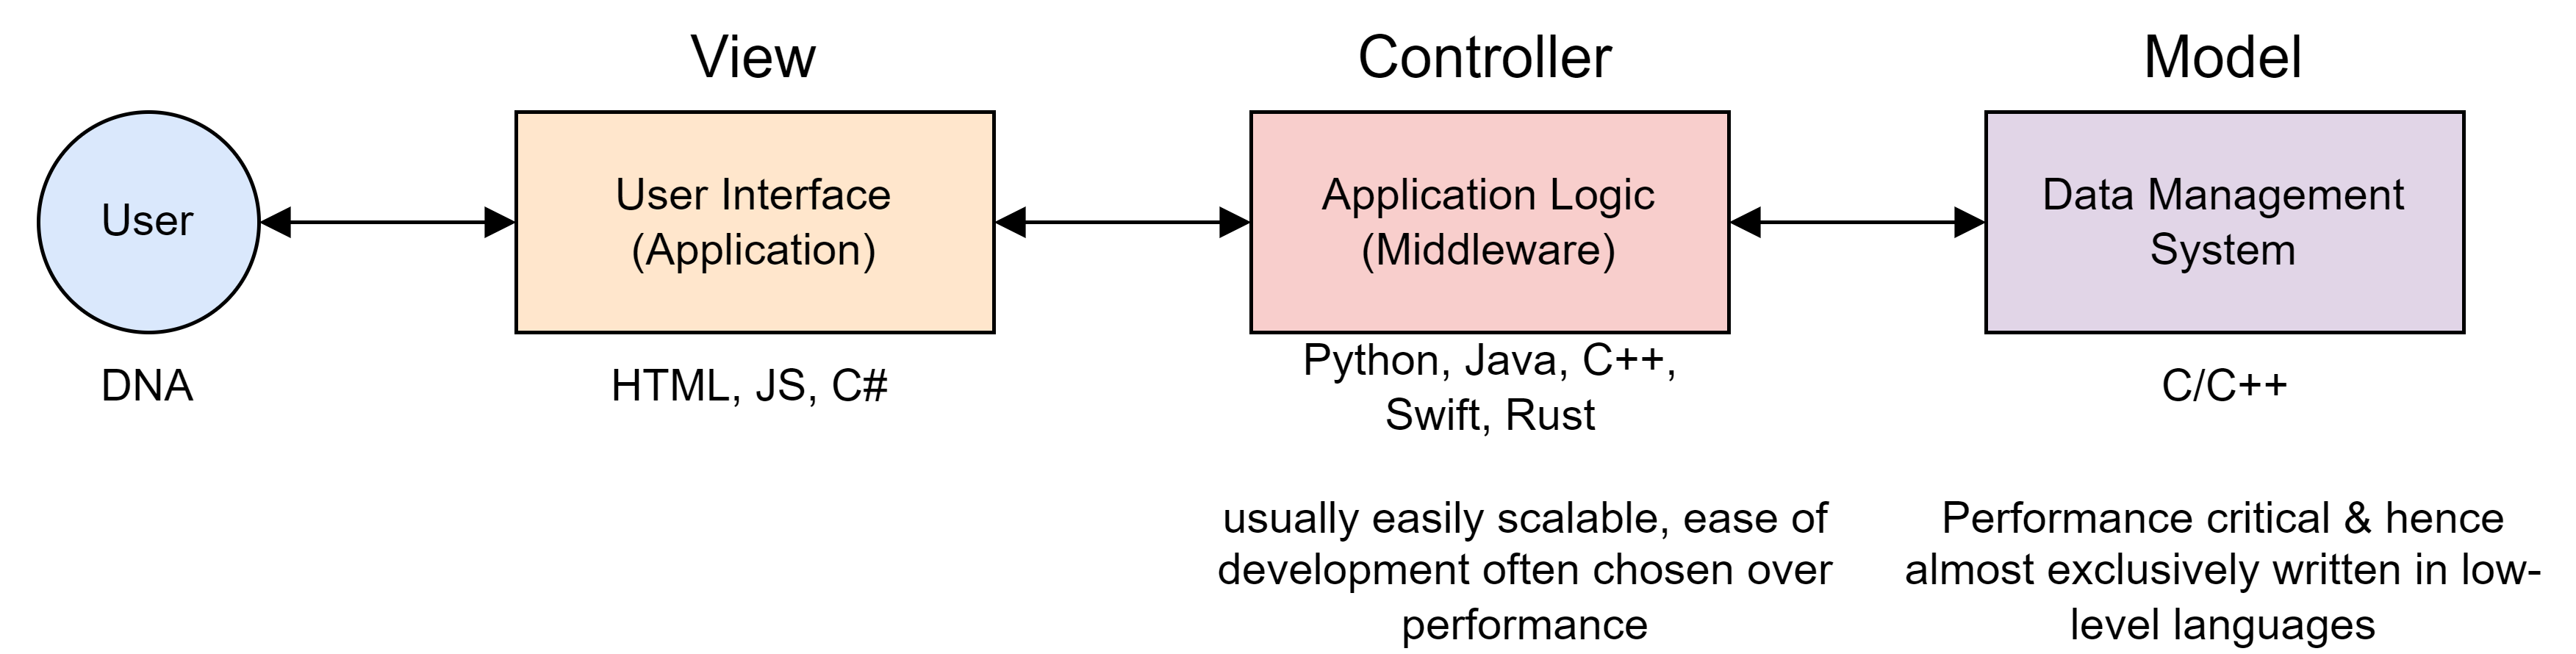
\includegraphics[width=.9\textwidth]{introduction/images/application_architecture.drawio.png}
\end{center}

\begin{sidenotebox}{Big Business}
    The enterprise data management systems market has been valued at $\$82.25$ billion (2021) with annual growth exceeding $10\%$ (\href{https://www.grandviewresearch.com/industry-analysis/enterprise-data-management-market}{grand view research}).
\end{sidenotebox}

\section{Data Management Systems}
\subsection{Non-Functional Requirements}
\begin{center}
    \begin{tabular}{l p{.8\textwidth}}
        \textbf{Efficiency}  & Ideally should be as fast as a bespoke, hand-written solution.                                                   \\
        \textbf{Resilience}  & Must be able to recover from failures (software crashes, power failure, hardware failure)                        \\
        \textbf{Robustness}  & Predictable performance (semantically small change in query $\Rightarrow$ similarly small change in performance) \\
        \textbf{Scalability} & Can scale performance with available resources.                                                                  \\
        \textbf{Concurrency} & Can serve multiple clients concurrently with a clear model for how concurrency will affect results.              \\
    \end{tabular}
\end{center}

\subsection{Logical/Physical Data Model Separation}
\begin{center}
    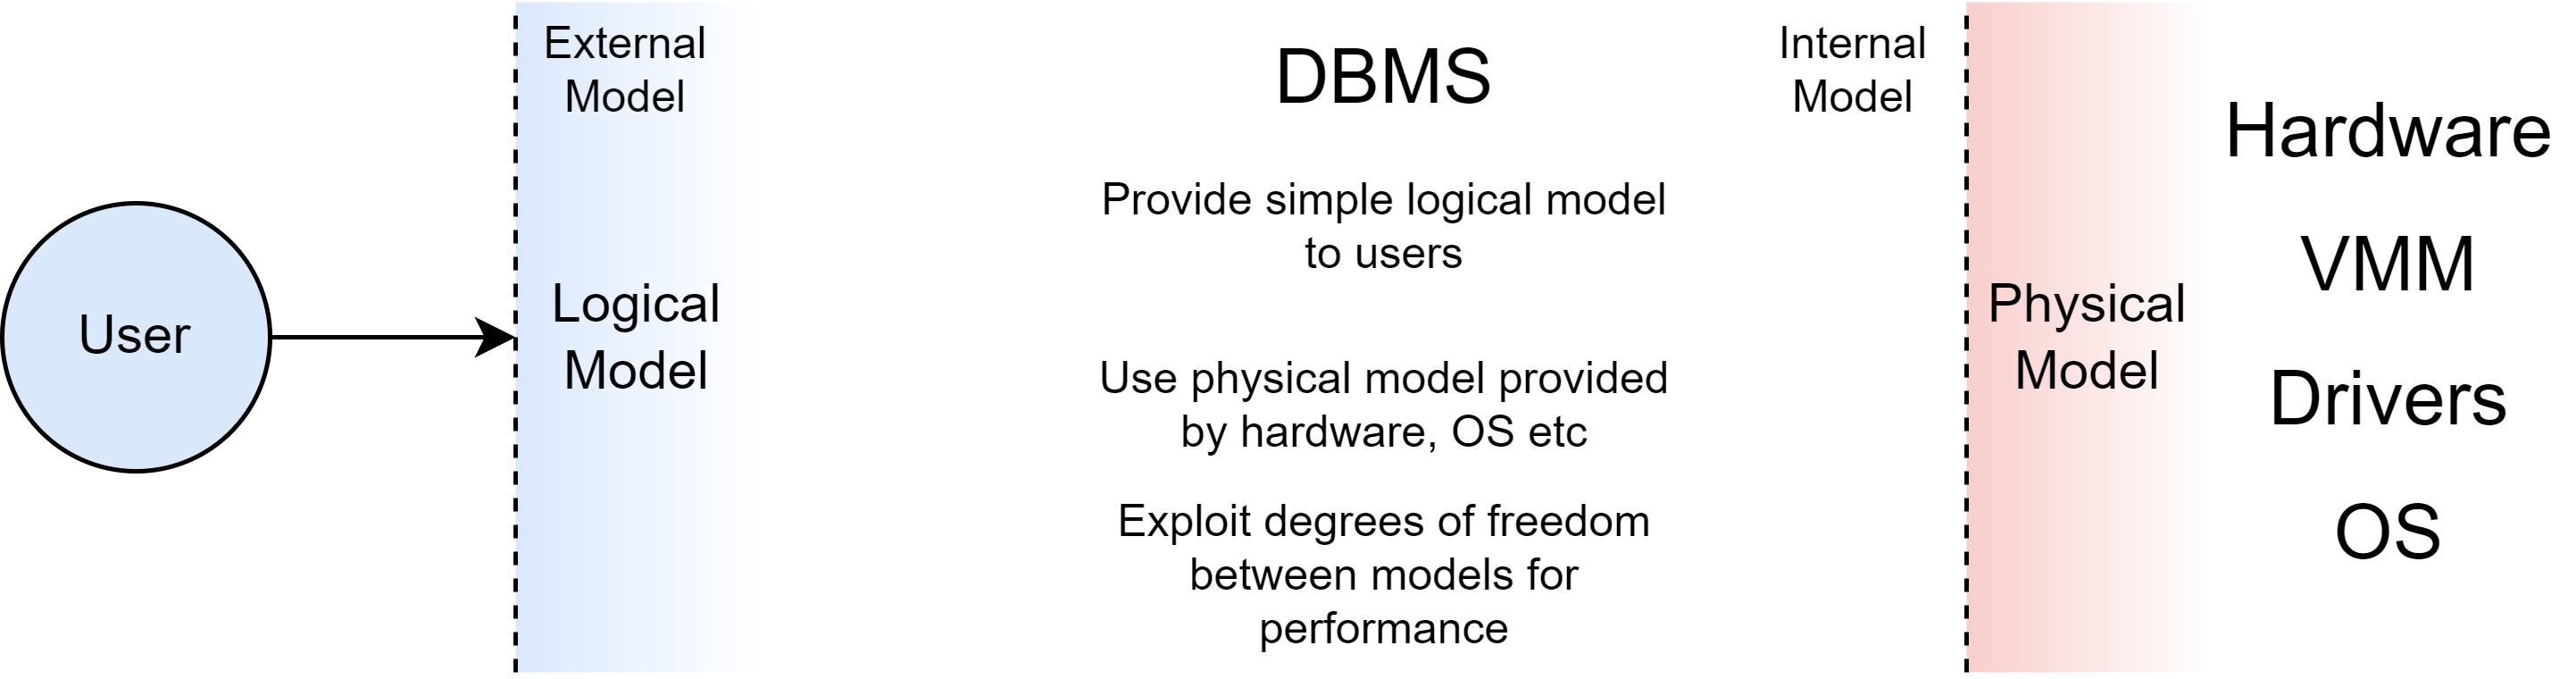
\includegraphics[width=.8\textwidth]{introduction/images/model_separation.drawio.png}
\end{center}

\subsection{Transactional Concurrency}

Actions to be performed on a data management system can be wrapped up as a \textit{transaction} to be received, processed and committed.

\begin{definitionbox}{ACID}
    A set of useful properties for database management systems.
    \begin{center}
        \begin{tabular}{l p{.8\textwidth}}
            \textbf{Atomic}     & A transaction either runs entirely (and is committed) or has no effect. (All or nothing)                                                                                             \\
            \textbf{Consistent} & A transaction can only bring the database from one valid (for some invariants) state to another. Note that there may be inconsistency between.                                       \\
            \textbf{Isolated}   & Many transactions run concurrently, however each leaves the database in some state equivalent to running the transactions in some sequential order. (Run as if alone on the system). \\
            \textbf{Durable}    & Once a transaction is committed, it is persistent (even in case of failure - e.g power failure).                                                                                     \\
        \end{tabular}
    \end{center}
\end{definitionbox}
\begin{center}
    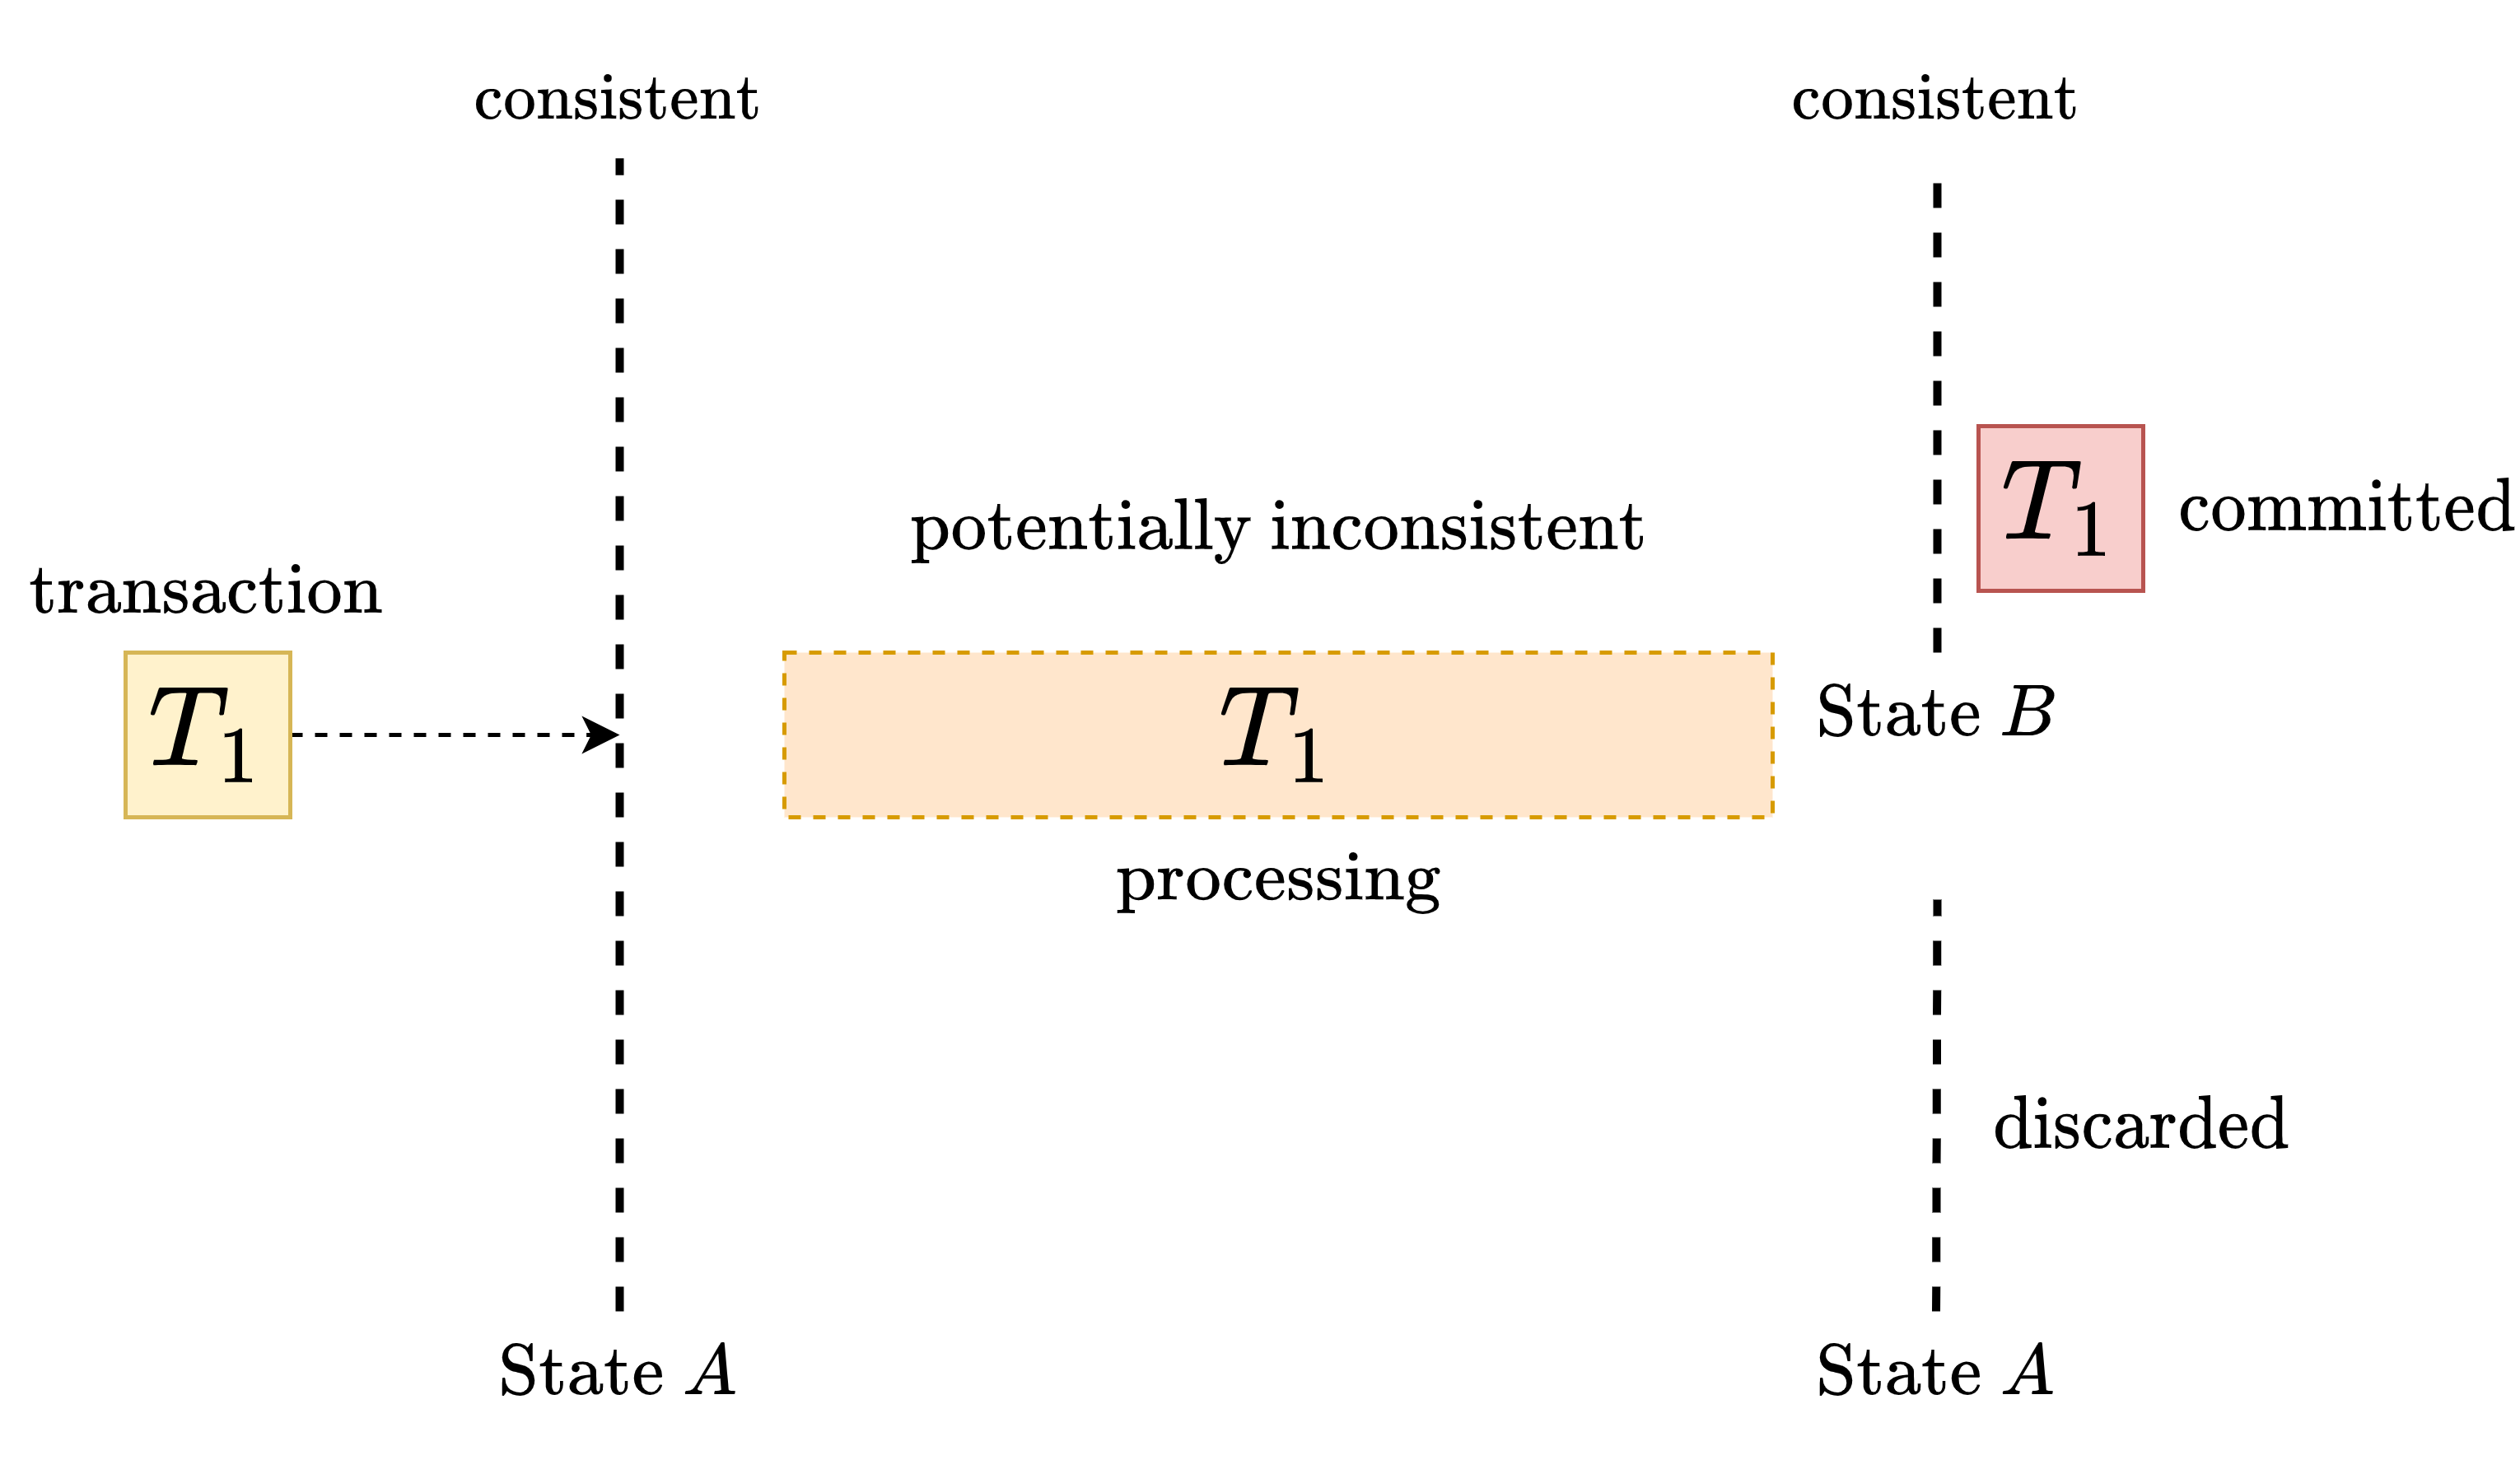
\includegraphics[width=.7\textwidth]{introduction/images/consistent_state.drawio.png}
\end{center}
\noindent
\textit{"Isolated"} is the most flexible ACID property, several \textit{isolation levels} describe how concurrent transactions interact.
The more isolation is enforced, the more locking is required which can affect performance (contention \& blocking).

\begin{sidenotebox}{Concurrency Controls}
    In order to support efficient concurrent access \& mutation of data without race conditions concurrency control is used:
    \begin{center}
        \begin{tabular}{l p{.8\textwidth}}
            Lock Based                                                                          & Each object (e.g record, table) contains a lock (read-write) used for synchronisation of access. The most common technique is \href{https://en.wikipedia.org/wiki/Two-phase_locking}{\textit{two-phase locking}}. \\
            \href{https://en.wikipedia.org/wiki/Multiversion_concurrency_control}{Multiversion} & Each object and transaction is timestamped, by maintaining multiple timestamped versions of an object a transaction can effectively operate on a snapshot of the database at its own timestamp.                   \\
        \end{tabular}
    \end{center}
    Concurrency control is discussed in detail in \autoref{chap:transactions}.
\end{sidenotebox}

\subsection{Read Phenomena}
You should already be familiar with some basic anomalies/phenomena, these include:
\begin{definitionbox}{Dirty Read / Uncommitted Dependency}
    A transaction reads a record updated by a transaction that has not yet committed.
    \begin{itemize}
        \item The uncommitted transaction may fail or be rolled back rendering the dirty-read data invalid.
    \end{itemize}
\end{definitionbox}
\begin{tcbraster}[raster columns=2, raster equal height]
    \begin{definitionbox}{Non-Repeatable Read}
        When a transaction reads a record twice with different results (another committed transaction updated the row between the reads).
    \end{definitionbox}
    \begin{definitionbox}{Phantom Reads}
        When a transaction reads a set of records twice, but the sets of records are not equal as another transaction committed between the reads.
    \end{definitionbox}
\end{tcbraster}
\subsection{Isolation levels}
\begin{definitionbox}{Serialisable}
    \begin{center}
        \begin{tabular}{c | c | c}
            \textit{Dirty Read}        & \textit{Non-repeatable Read} & \textit{{Phantom Read}}    \\
            \textcolor{red}{Prevented} & \textcolor{red}{Prevented}   & \textcolor{red}{Prevented} \\
        \end{tabular}
    \end{center}
    Execution of transactions is can be serialized (it is equivalent to some sequential history of transactions).
    \begin{itemize}
        \item In lock-based concurrency control locks are released at the end of a transaction, and range-locks are acquired for \mintinline{sql}{SELECT ... FROM ... WHERE ... ;} to avoid \textit{phantom reads}.
        \item Prevents all 3 read phenomena and is the strongest isolation level.
    \end{itemize}
\end{definitionbox}
\begin{definitionbox}{Repeatable Reads}
    \begin{center}
        \begin{tabular}{c | c | c}
            \textit{Dirty Read}        & \textit{Non-repeatable Read} & \textit{{Phantom Read}}          \\
            \textcolor{red}{Prevented} & \textcolor{red}{Prevented}   & \textcolor{ForestGreen}{Allowed} \\
        \end{tabular}
    \end{center}
    \begin{itemize}
        \item Unlike \textit{serialisable} Range locks are not used, only locks per-record.
        \item Write skew can occur (when concurrent transactions write to the same table \& column using data read from the table, resulting in a mix of both transactions)
    \end{itemize}
\end{definitionbox}
\begin{definitionbox}{Read Committed}
    \begin{center}
        \begin{tabular}{c | c | c}
            \textit{Dirty Read}        & \textit{Non-repeatable Read}     & \textit{{Phantom Read}}          \\
            \textcolor{red}{Prevented} & \textcolor{ForestGreen}{Allowed} & \textcolor{ForestGreen}{Allowed} \\
        \end{tabular}
    \end{center}
    Mutual exclusion is held for writes, but reads are only exclusive until the end of a \mintinline{sql}{SELECT ... ;} statement, not until commit time.
    \begin{itemize}
        \item In lock-based concurrency, write locks are held until commit, read locks released after select completed.
    \end{itemize}
\end{definitionbox}
\begin{definitionbox}{Read Uncommitted}
    \begin{center}
        \begin{tabular}{c | c | c}
            \textit{Dirty Read}              & \textit{Non-repeatable Read}     & \textit{{Phantom Read}}          \\
            \textcolor{ForestGreen}{Allowed} & \textcolor{ForestGreen}{Allowed} & \textcolor{ForestGreen}{Allowed} \\
        \end{tabular}
    \end{center}
    The weakest isolation level and allows for all \textit{read phenomena}.
\end{definitionbox}

\subsection{Declarative Data Analysis}
In order to make complex data management tools easier to use, a programmer describes the result
they need declaratively, and the database system then plans the operations that must occur to
provide the requested result.
\\
\\ This is present in almost all databases (e.g SQL \& SQL derived languages).
